\section{Background}
This section reviews R{\'e}nyi's $\alpha$-divergence and variational inference upon which the new framework is based. Note that there exist other $\alpha$-divergence definitions \citep{amari:divergence, tsallis:divergence} (see appendix). However we mainly focus on R{\'e}nyi's definition as it enables us to derive a new class of variational lower-bounds.

\subsection{R{\'e}nyi's $\alpha$-divergence}

\label{sec:renyi_divergence}
We first review R{\'e}nyi's $\alpha$-divergence \cite{renyi:divergence, van_erven:renyi}. R{\'e}nyi's $\alpha$-divergence, defined on $\{\alpha: \alpha > 0, \alpha \neq 1, |\mathrm{D}_{\alpha}| < +\infty \}$, measures the ``closeness'' of two distributions $p$ and $q$ on a random variable $\bm{\theta} \in \Theta$:
\begin{equation}
\label{eq:renyi_divergence}
\mathrm{D}_{\alpha} [p || q] = \frac{1}{\alpha - 1} \log \int p(\bm{\theta})^{\alpha} q(\bm{\theta})^{1 - \alpha} d \bm{\theta}.
\end{equation}
The definition is extended to $\alpha = 0, 1, +\infty$ by continuity. We note that when $\alpha \rightarrow 1$ the Kullback-Leibler (KL) divergence is recovered, which plays a crucial role in machine learning and information theory. Some other special cases are presented in Table \ref{tab:renyi_example}. The method proposed in this work also considers $\alpha \leq 0$ (although (\ref{eq:renyi_divergence}) is no longer a divergence for these $\alpha$ values), and we include from \cite{van_erven:renyi} some useful properties for forthcoming derivations.
%
\begin{prop}
(Monotonicity) R{\'e}nyi's $\alpha$-divergence definition (\ref{eq:renyi_divergence}), extended to negative $\alpha$, is \textbf{continuous} and \textbf{non-decreasing} on $\alpha \in \{\alpha: -\infty < \mathrm{D}_{\alpha} < +\infty \}$.
\label{prop:renyi_divergence}
\end{prop}
%
\begin{prop}
(Skew symmetry) For $\alpha \not\in \{0, 1\}$, 
$
\mathrm{D}_{\alpha} [p || q] = \frac{\alpha}{1 - \alpha} \mathrm{D}_{1 - \alpha} [q || p].
$
This implies $\mathrm{D}_{\alpha} [p || q] \leq 0$ for $\alpha < 0$. For the limiting case $\mathrm{D}_{-\infty} [p || q] = -\mathrm{D}_{+\infty} [q || p]$.
\label{prop:skew_symmetry}
\end{prop}
%
%
\begin{table}[t]
  \centering
  \caption{Special cases in the R{\'e}nyi divergence family.}
  \renewcommand{\arraystretch}{1.2}
  \label{tab:renyi_example}
  \begin{tabular}{ccl}
  	\toprule
    $\alpha$ & Definition & Notes\\
    \hline
    $\alpha \rightarrow 1$ & $\int p(\bm{\theta}) \log \frac{p(\bm{\theta})}{q(\bm{\theta})} d \bm{\theta}$ & 
    \begin{tabular}{@{}l@{}} \emph{Kullback-Leibler (KL) divergence}, \\ used in VI ($\mathrm{KL}[q||p]$) and EP ($\mathrm{KL}[p||q]$) \end{tabular} \\
    %
    $\alpha = 0.5$ & $-2 \log (1 - \mathrm{Hel}^2[p||q])$ & function of the square \emph{Hellinger distance}\\
    %
    $\alpha \rightarrow 0$ & $-\log \int_{p(\bm{\theta}) > 0} q(\bm{\theta}) d\bm{\theta}$ & 
    \begin{tabular}{@{}l@{}} zero when $\mathrm{supp}(q) \subseteq \mathrm{supp}(p)$ \\ (not a divergence) \end{tabular} \\
    %
    $\alpha = 2$ & $-\log (1 - \chi^2[p||q])$ & 
    \begin{tabular}{@{}l@{}} proportional to the $\chi^2$-divergence \end{tabular} \\
    %
    $\alpha \rightarrow +\infty$ & $\log \max_{\bm{\theta} \in \Theta} \frac{p(\bm{\theta})}{q(\bm{\theta})}$ &
    \begin{tabular}{@{}l@{}} \emph{worst-case regret} in \\ \emph{minimum description length principle} \cite{grunwald:mdl}\end{tabular} \\
    \bottomrule
  \end{tabular}
  %\vspace{-0.1in}
\end{table}
%
A critical question that is still in active research is how to choose a divergence in this rich family to obtain optimal solution for a particular application, an issue which is discussed in the appendix.

\subsection{Variational inference}
\label{sec:vi}
Next we review the variational inference algorithm \cite{jordan:vi, beal:thesis} using posterior approximation as a running example.
%
Consider observing a dataset of $N$ i.i.d.~samples $\mathcal{D} = \{\bm{x}_n \}_{n=1}^N$ from a probabilistic model $p(\bm{x}|\bm{\theta})$ parametrised by a random variable $\bm{\theta}$ that is drawn from a prior $p_0(\bm{\theta})$. Bayesian inference involves computing the posterior distribution of the parameters given the data, 
\begin{equation}
p(\bm{\theta} | \mathcal{D}, \bm{\varphi}) = \frac{p(\bm{\theta}, \mathcal{D}| \bm{\varphi})}{p(\mathcal{D}| \bm{\varphi})} = \frac{p_0(\bm{\theta}| \bm{\varphi}) \prod_{n=1}^{N} p(\bm{x}_n | \bm{\theta}, \bm{\varphi})}{p(\mathcal{D}| \bm{\varphi})}, 
\end{equation}
where $p(\mathcal{D}| \bm{\varphi}) = \int p_0(\bm{\theta}| \bm{\varphi}) \prod_{n=1}^{N} p(\bm{x}_n | \bm{\theta}, \bm{\varphi}) d\bm{\theta}$ is called marginal likelihood or model evidence. The hyper-parameters of the model are denoted as $\bm{\varphi}$ which might be omitted henceforth for notational ease. 
%
For many powerful models the exact posterior is typically intractable, and approximate inference introduces an approximation $q(\bm{\theta})$ in some tractable distribution family $\mathcal{Q}$ to the exact posterior. One way to obtain this approximation is to minimise the KL divergence $\mathrm{KL}[q(\bm{\theta}) || p(\bm{\theta} | \mathcal{D})]$, which is also intractable due the difficult term $p(\mathcal{D})$. Variational inference (VI) sidesteps this difficulty by considering an equivalent optimisation problem that maximises the \emph{variational lower-bound}:
\begin{equation}
\mathcal{L}_{\text{VI}}(q; \mathcal{D}, \bm{\varphi}) = \log p(\mathcal{D}|\bm{\varphi}) - \mathrm{KL}[q(\bm{\theta}) || p(\bm{\theta} | \mathcal{D}, \bm{\varphi})]
	= \mathbb{E}_{q} \left[ \log  \frac{p(\bm{\theta}, \mathcal{D}|\bm{\varphi})}{q(\bm{\theta})} \right].
\label{eq:vi_bound}
\end{equation}
The variational lower-bound can also be used to optimise the hyper-parameters $\bm{\varphi}$.

%
To illustrate the approximation quality of VI we present a mean-field approximation example to Bayesian linear regression in Figure \ref{fig:linear_regression_posterior} (in magenta). Readers are referred to the appendix for details, but essentially a factorised Gaussian approximation is fitted to the true posterior, a correlated Gaussian in this case. The approximation recovers the posterior mean correctly, but is over-confident. Moreover, as $\mathcal{L}_{\text{VI}}$ is the difference between the marginal likelihood and the KL divergence, hyper-parameter optimisation can be biased away from the exact MLE towards the region of parameter space where the KL term is small \cite{turner:two_problems} (see Figure \ref{fig:linear_regression_energy}). 

\begin{figure}[t]
 \centering
 \subfigure[Approximated posterior.]{
 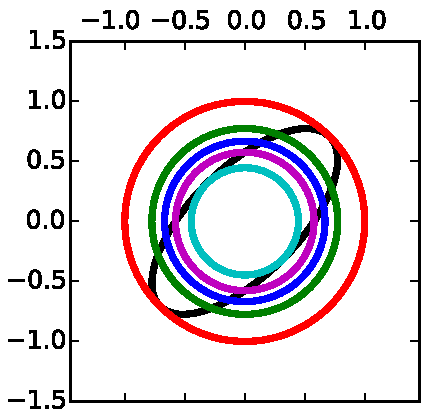
\includegraphics[width=0.24\linewidth]{figs/approx.pdf}
 \label{fig:linear_regression_posterior}}
 \hspace{0.5in}
 \subfigure[Hyper-parameter optimisation.]{
 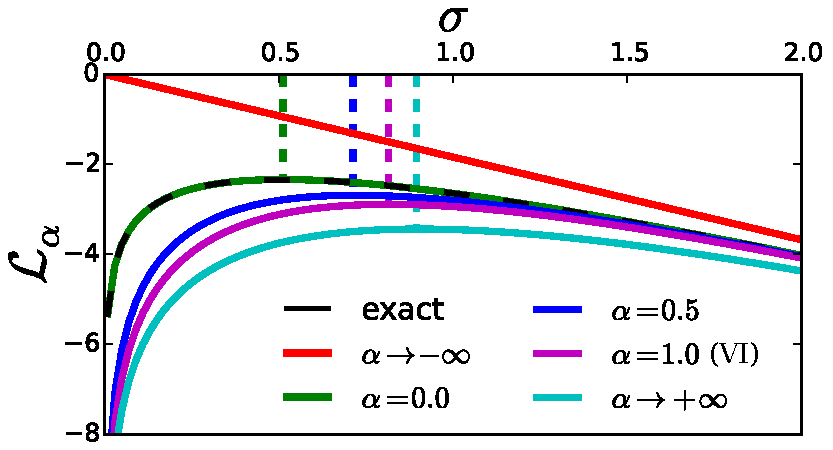
\includegraphics[width=0.45\linewidth]{figs/log_evidence.pdf}
 \label{fig:linear_regression_energy}}
 %\vspace{-0.1in}
 \caption{Mean-Field approximation for Bayesian linear regression. In this case $\bm{\varphi} = \sigma$ the observation noise variance. The bound is tight as $\sigma \rightarrow +\infty$, biasing the VI solution to large $\sigma$ values.}
\end{figure}